% Slide 12 | Results | M5 (Saatwik Tiwari) | 1:15 | E3: is Bertram's formula right?
\begin{frame}{E3: the formula is right, daily checking is slower}
\framesubtitle{Slide 12 \textbullet\ Results \textbullet\ M5 \textbullet\ 1:15}
\vspace{-2pt}
\begin{columns}[T,onlytextwidth]
\column{0.50\textwidth}
  \centering
  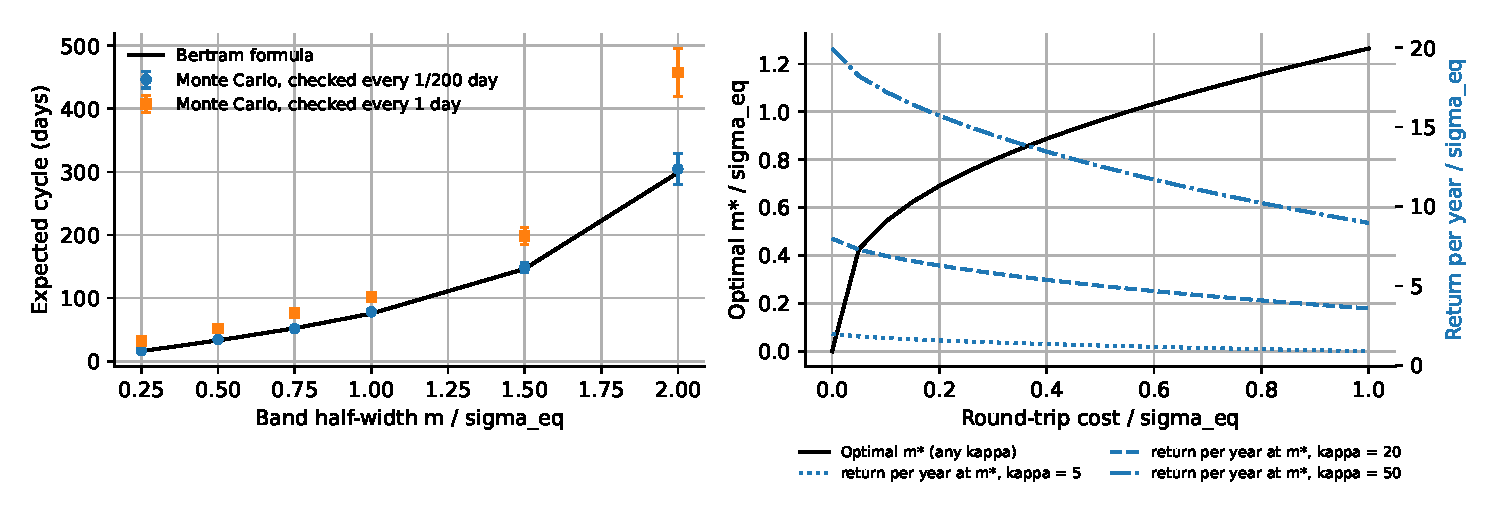
\includegraphics[width=\linewidth,trim=0bp 0bp 374bp 0bp,clip]{fig_e3_bertram}\\[1pt]
  {\scriptsize expected cycle time: formula against simulation}
\column{0.46\textwidth}
  \footnotesize\raggedright
  \begin{itemize}\setlength{\itemsep}{3pt}
    \item the formula is \textbf{exact}: it matches a numerical integration to $10^{-8}$
    \item checking prices once a day makes a cycle \textbf{35--99\% longer}
  \end{itemize}
\end{columns}
\pairTakeaway{The spread can cross a band and return between two daily looks.}
\end{frame}
